\chapter{Datasets for Acoustic Echo Estimation \& \dechorate}\label{chap:ch:dechorate}

\openepigraph{Signal, a function that conveys information about a phenomenon.
$[\dots]$ Consider an acoustic wave, which can convey acoustic or music information.}{R. Priemer, \textit{Introductory Signal Processing}}
\vspace{-2.5em}

\newthought{Synopsis}
This paper presents \dEchorate{}: a new database of measured multichannel room impulse response (RIRs) including annotations of early echoes and 3D positions of microphones, real and image sources under different wall configurations in a cuboid room.
These data provide a tool for benchmarking recent methods in \textit{echo-aware} speech enhancement, room geometry estimation, RIR estimation, acoustic echo retrieval, microphone calibration, echo labeling and reflectors estimation.
The database is accompanied with software utilities to easily access, manipulate and visualize the data as well as baseline methods for echo-related tasks. The database is publicly available at \linkDechorate

\section{Introduction}\label{sec:dechorate:intro}

When sound travels from a source to a microphone in a indoor environment, it interacts with it by being delayed and attenuated due to the distance; reflected, absorbed and diffracted due to the surfaces. The room impulse response (RIR) translates this phenomenon as a linear and causal time-domain filter.
As depicted in Fig.~\ref{fig:rir}, RIRs are commonly subdivided into 3 parts:
the \textit{direct-path}, corresponding to the line-of-sight; the \textit{early echoes}, stemming from few disjoint reflections on the closest reflectors; and the \textit{reverberation tail} comprising the dense accumulation of late reflections and  \textit{scattering} effects. While the reverberation perceptually corresponds to the ``liveliness'' and naturalness of sounds \cite{geldard1953human}, the times of arrival (TOAs) of the direct path and early echoes carry precise information on the scene's geometry \cite{Kuttruff2009room}. Such relation is well explained by the image source model (ISM) \cite{Allen1979image}, where the echoes are associated with the contribution of virtual sound sources lying outside the real room.

\begin{figure}
    \centering
    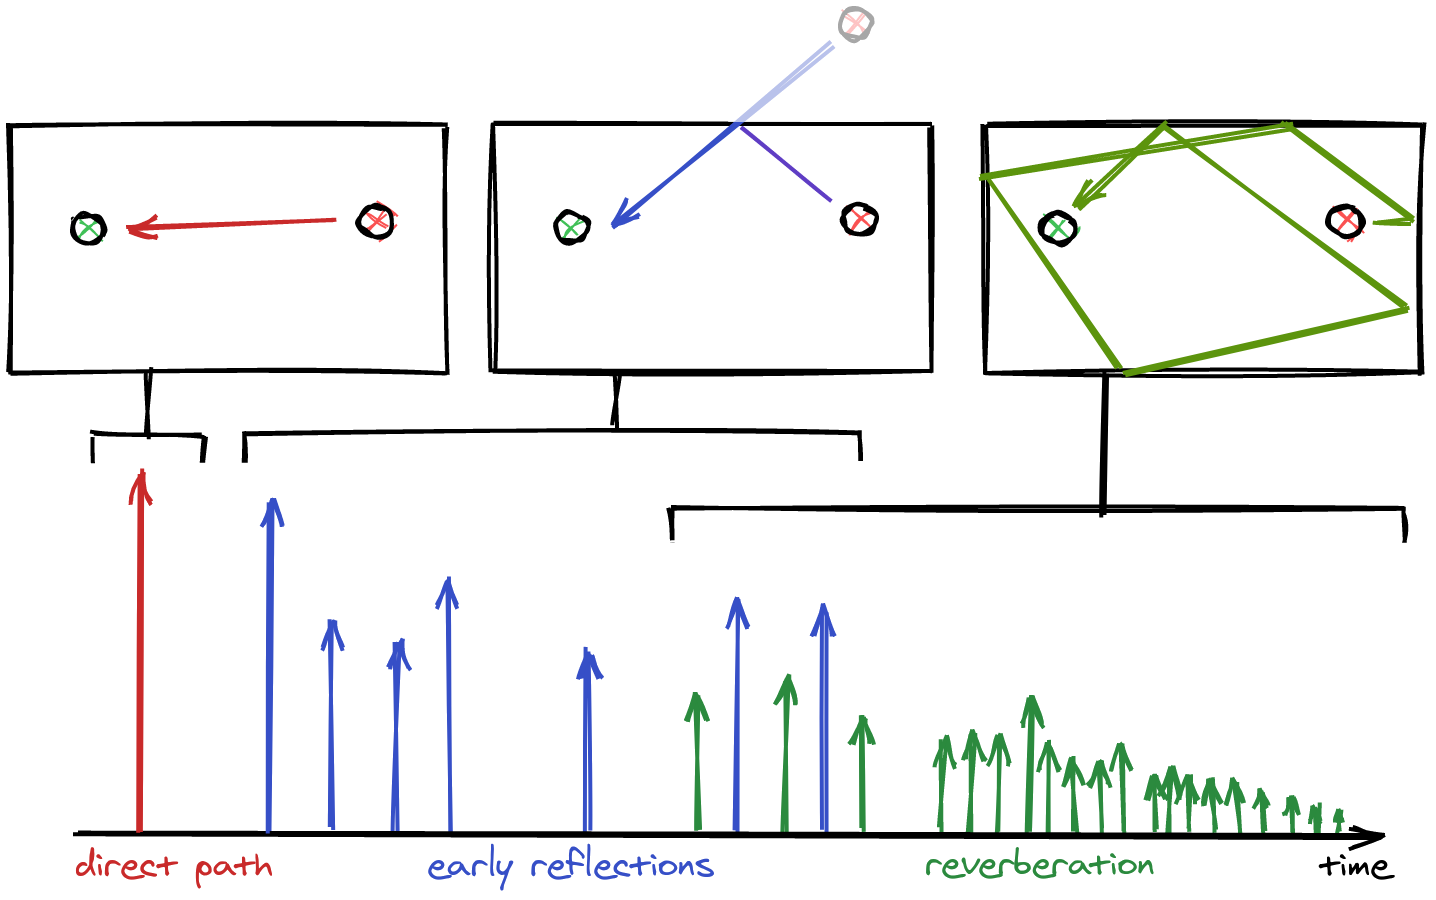
\includegraphics[width=\linewidth]{dechorate/rir_model_empty.png}
    \caption{Depiction of the different components of a room impulse response as they relate to sound propagation.}
    \label{fig:rir}
\end{figure}


% Please add the following required packages to your document preamble:
% \usepackage{multirow}
\begin{table*}[h!]
\label{tab:rir_db}
\small
\centering

\begin{tabular}{l|c|c|c|ccc|c|l|l}
\toprule

\multirow{2}{*}{Database Name} &
  \multicolumn{3}{c|}{Annotated} &
  \multicolumn{4}{c|}{Number of} &
  Key characteristics &
  Purpose \\
  &
  Pos. &
  Echoes &
  Rooms &
  \multicolumn{1}{l|}{RIRs} &
  \multicolumn{1}{c|}{Rooms} &
  \multicolumn{1}{c|}{Mic$\times$Pos.} &
  Src &
   &
   \\
\hline
\begin{tabular}[c]{@{}l@{}} Dokmani\'c \textit{et al.} \citeonly{Dokmanic2013acoustic}\end{tabular} &
  \cmark  &
  $\sim$ &
  \multicolumn{1}{c|}{$\sim$} &
  \multicolumn{1}{l|}{15} &
  \multicolumn{1}{c|}{3} &
  \multicolumn{1}{c|}{5} &
  1 &
  Non shoebox room &
  RooGE \\ \hline
\begin{tabular}[c]{@{}l@{}} Crocco \textit{et al.} \citeonly{crocco2017uncalibrated}\end{tabular} &
  \cmark &
  $\sim$ &
  \multicolumn{1}{c|}{\cmark} &
  \multicolumn{1}{l|}{204} &
  \multicolumn{1}{c|}{1} &
  \multicolumn{1}{c|}{17} &
  12 &
  \begin{tabular}[c]{@{}l@{}}Accurate 3D calibration\\ Many mic and src positions\end{tabular} &
  RooGE \\
 \hline

 Remaggi \textit{et al.} \citeonly{remaggi2016acoustic} &
  \cmark & % # noete pos?
  $\sim$  & % # note echo?
  \cmark & % # note room?
  \multicolumn{1}{l|}{$\sim$1.5k} & % # rirs
  \multicolumn{1}{c|}{4} & % # room
  \multicolumn{1}{c|}{48$\times$2} & % # mics
  4-24 & % # srcs
  \begin{tabular}[c]{@{}l@{}}
  Circural dense array
  \\Circular placement of sources
  \end{tabular} &
  \begin{tabular}[c]{@{}l@{}}RooGE\\ SE$^{\dagger}$\end{tabular}
  \\
\hdashline
Remaggi \textit{et al.} \citeonly{Remaggi2019modeling} &
  \cmark & % # noete pos?
  $\sim$  & % # note echo?
  \cmark & % # note room?
  \multicolumn{1}{l|}{$\sim$1.6k} & % # rirs
  \multicolumn{1}{c|}{4} & % # room
  \multicolumn{1}{c|}{
    \begin{tabular}[c]{@{}l@{}}
    48$\times$2
    \\+2$\times$2
    \end{tabular}
} & % # mics
  3-24 & % # srcs
  \begin{tabular}[c]{@{}l@{}}
    Circural dense array
    \\Binaural Recordings
    \end{tabular}
  &
  \begin{tabular}[c]{@{}l@{}}RooGE$^{\dagger}$\\ SE\end{tabular}
  \\
\hline
BUT Reverb dB \citeonly{Szoke2018building} &
  \cmark &
  \xmark&
  $\sim$ &
  \multicolumn{1}{l|}{$\sim$1.3k} &
  \multicolumn{1}{c|}{8} &
  \multicolumn{1}{c|}{(2-10)$\times$6} &
  3-11 &
  \begin{tabular}[c]{@{}l@{}}Accurate metadata\\ different device/arrays\\ various rooms\end{tabular} &
  SE/ASR \\ \hline
VoiceHome \citeonly{Bertin2019voice} &
   \cmark &
   \xmark&
   \xmark&
  \multicolumn{1}{l|}{188} &
  \multicolumn{1}{c|}{12} &
  \multicolumn{1}{c|}{8$\times$2} &
  7-9  &
   Various rooms, real homes &
  SE/ASR \\ \hline
dEchorate &
  \textbf{\cmark} &
  \textbf{\cmark} &
  \multicolumn{1}{c|}{\textbf{\cmark}} &
  \multicolumn{1}{l|}{$\sim$1.8k} &
  \multicolumn{1}{c|}{1} &
  \multicolumn{1}{c|}{30} &
  6 &
  \begin{tabular}[c]{@{}l@{}}Accurate annotation\\ Different Echo-energy\end{tabular} &
  \begin{tabular}[c]{@{}l@{}}RooGE\\ SE/ASR\end{tabular}
  \\

\bottomrule
\end{tabular}
\caption{Comparison between some existing RIR databases that account for early acoustic reflections. Receiver positions are indicated in terms of number of microphones per array times number of different positions of the array ($\sim$ stands for partially available information).
The read is invited to refer to \citeonly{Szoke2018building, Genovese2019blind} for more complete list of existing RIR datasets.
%\protect\\- indicates minimum and maximum number of variable number of objects
\protect\\$^{\dagger}$The dataset in \citeonly{remaggi2016acoustic} is originally intended for RooGE and further extended for (binaural) SE in \citeonly{Remaggi2019modeling} with a similar setup.}
\end{table*}

Based on this idea, so-called \textit{echo-aware} methods have been introduced few decades ago, where matched filters (or rake receivers) are used to constructively sum the sound reflections \cite{Jan1995matched, Affes1997signal} and build beamformers achieving much better sound qualities \cite{Gannot2001signal}. This methods have recently regained interested as manifested by the European project SCENIC~\cite{Annibale2011scenic} and the UK research \href{http://www.s3a-spatialaudio.org/}{S$^3$A project}. They show that knowing the properties of a few early echoes can boosts performances of typical indoor audio inverse problems such as speech enhancement (SE) \cite{Dockmanic2015raking, Kowalczyk2019raking}, sound source localization \cite{Ribeiro2010turning, DiCarlo2019mirage}, and separation \cite{Scheibler2017separake, Leglaive2016multichannel}.

Another fervent area of research spanning transversely the audio and acoustic signal processing fields is estimating the room geometry blindly from acoustic signals. As presented by Crocco \textit{et al.} in \cite{Crocco2017uncalibrated}, the end-to-end room geometry estimation (RooGE) involves many subsequent subtasks: RIR estimation, peak picking, microphones calibration, echo labeling, reflectors estimation. Acoustic echo retrieval (AER) is common to many of these topics. It consists in estimating the properties of echoes such as their TOAs and energies. The former problem is referred to as TOA estimation, or time-delay estimation when the direct-path is taken as reference. Furthermore, as interesting applications, these methods have been recently used in active scenarios, namely knowing the transmitted signals, using unmanned aerial vehicle (UAV, a.k.a. drones) \cite{Jensen2019method, Boutin2020drone} and mobile-phones \cite{Shih2019phone}.

As listed in \cite{Szoke2018building} and in \cite{Genovese2019blind}, a number of recorded RIRs corpora are available online and for free, each of them meeting the demands of certain applications, usually SE and ASR. However, even if these datasets feature reverberation and strong reflections, they lack proper annotations, making them difficult to use for echo-aware tasks. For this reason, to bypass the complexity of recording real annotated RIR datasets, simulators based on the ISM are extensively used instead~\cite{Gaultier2017vast, Kim2017generation, Perotin2018crnn}. While simulated datasets are more versatile, simple and quicker to obtain, they fail to fully capture the complexity and the richness of real acoustic environments. Due to this, methods trained or validated on them may fail to generalize to real conditions, as will be shown in this paper. Interestingly, the authors of \cite{Genovese2019blind} fused together multiple real and synthetic dataset in order to find a balance between number of training data and realism.

A good echo-oriented RIR dataset should include a variety of environments (rooms geometries and surface materials), of microphone placings (close to or away from reflectors, scattered or forming ad-hoc arrays) and, most importantly, precise annotations of the scene's geometry and echo timings in the RIRs. Moreover, in order to be versatile and used in both SE and RooGE applications, the provided annotations should match the ISM, \textit{i.e.}, TOAs should be expressed in terms of image sources and vice-versa. Such data are difficult to collect since they require precise measurements of the positions and orientations of all the acoustic emitters, receivers and reflective surfaces inside the environment with dedicated planimetric equipment. We identified two main classes of related RIR datasets in the literature: SE/ASR-oriented datasets, e.g. \cite{Szoke2018building, Bertin2019voice, Cmejla2019mirage}, and RooGE-oriented datasets, e.g. \cite{Dokmanic2013acoustic, Crocco2017uncalibrated, remaggi2017acoustic}. The formers include acoustic echoes as highly correlated interfering source coming from close reflectors, such as desk in meeting rooms or the close wall, however their proper annotations are not provided. The latter group deals with sets of distributed, synchronized microphones and loudspeakers in a room. These setups are not exactly suitable for SE methods, which typically involve compact or ad hoc arrays. Table~\ref{tab:rir_db} summarizes some existing datasets.

To fill this gap, we present \dEchorate{}: a fully calibrated multichannel RIR database with accurate annotation of the geometry and echoes in different configurations of a cuboid rooms with varying wall acoustic profiles.
The database currently features 1800 annotated RIRs obtained from 6 arrays of 5 microphones each, 6 sound sources in 10 different acoustic conditions. All the measurements were realized in the acoustic lab at Bar-Ilan university following a consolidated protocol previously established for the realization of two other multichannel RIRs databases: the BIU's Impulse Response Database \cite{Hadad2014multichannel} gathering RIRs of different reverberation levels sensed by uniform linear arrays (ULAs); and \texttt{MIRaGE} \cite{Cmejla2019mirage} providing a set of measurements for a source position that can be place in in dense position grid. \dEchorate{} is designed for AER with linear arrays, and is more generally aimed at analysing and benchmarking RooGE and echo-aware signal processing methods on real data. In particular, it can be used to assess robustness against the number of reflectors, the reverberation time, additive spatially-diffuse noise and non-ideal frequency and directive characteristics of microphone-source pairs and surfaces in a controlled way. Due to the amount of data and recording conditions, it could also be used to train machine learning models or as a reference to improve RIR simulators.

The database is accompanied with a Python toolbox that can be used to process and visualize the data,  perform analysis or to annotate new datasets.

\section{Database Description}

\begin{table}[]
    \centering
    \small
    \begin{tabular}{ll}
        \toprule
         Loudspeakers   & (directional, direct) $4 \times$ Avanton\\
                        & (directional, indirect) $2 \times$ Avanton\\
                        & (omnidirectional) $1 \times$ B\&G\\
                        & (babble noise) $4 \times$ 6301bx Fostex\\
         \hline
         Microphones    & $30 \times$ AKG CK32\\
         Array          & $6 \times$ nULA (5 mics each, handcrafted)\\
         \hline
         A/D Converter  & ANDIAMO.MC\\
         \hline
         Indoor Positioning & Marvelmind Starter Set HW v4.9\\
         \bottomrule
    \end{tabular}
    \caption{Measurements equipment.}
    \label{tab:room_equipment}
\end{table}

\subsection{Recording setup}
The recording setup is situated in a cuboid room with dimension 6 m $\times$ 6 m $\times$ 2.4 m. The 6 facets of the room (walls, ceiling, floor) are covered by acoustic panels allowing controllable reverberation time ($\RT$). We placed $4$ directional loudspeakers (direct sources) facing the center of the room and $30$ microphones mounted on $6$ non-uniform linear arrays (nULA) of $5$ sensors each. An additional channel is used for the loop-back signal, which serves to compute the time of emission and detect errors. Each loudspeaker and each array was positioned close to one of the walls in such a way that the nature of the strongest echo can is easily identifiable. Moreover, their positioning was chosen to cover a wide distribution of source-to-receiver distances, hence, a wide range of direct-to-reverberant ratio (DRR). Further, $2$ more loudspeakers were positioned pointing towards the walls (indirect sources). This was done to study the case of early reflections being stronger than the direct-path.

Each linear microphone arrays consists in $5$ microphones with non-unifor inter-microphone spacings of $[4, 5, 7.5, 10]$ cm\sidenote{\textit{i.e.} $[-12.25, -8.25, -3.25, 3.25, 13.25]$ cm w.r.t the barycenter}. Each array is steered towards a different vertical edge of the room for calibration and reproducibility purposes.

\begin{figure}
    \centering
    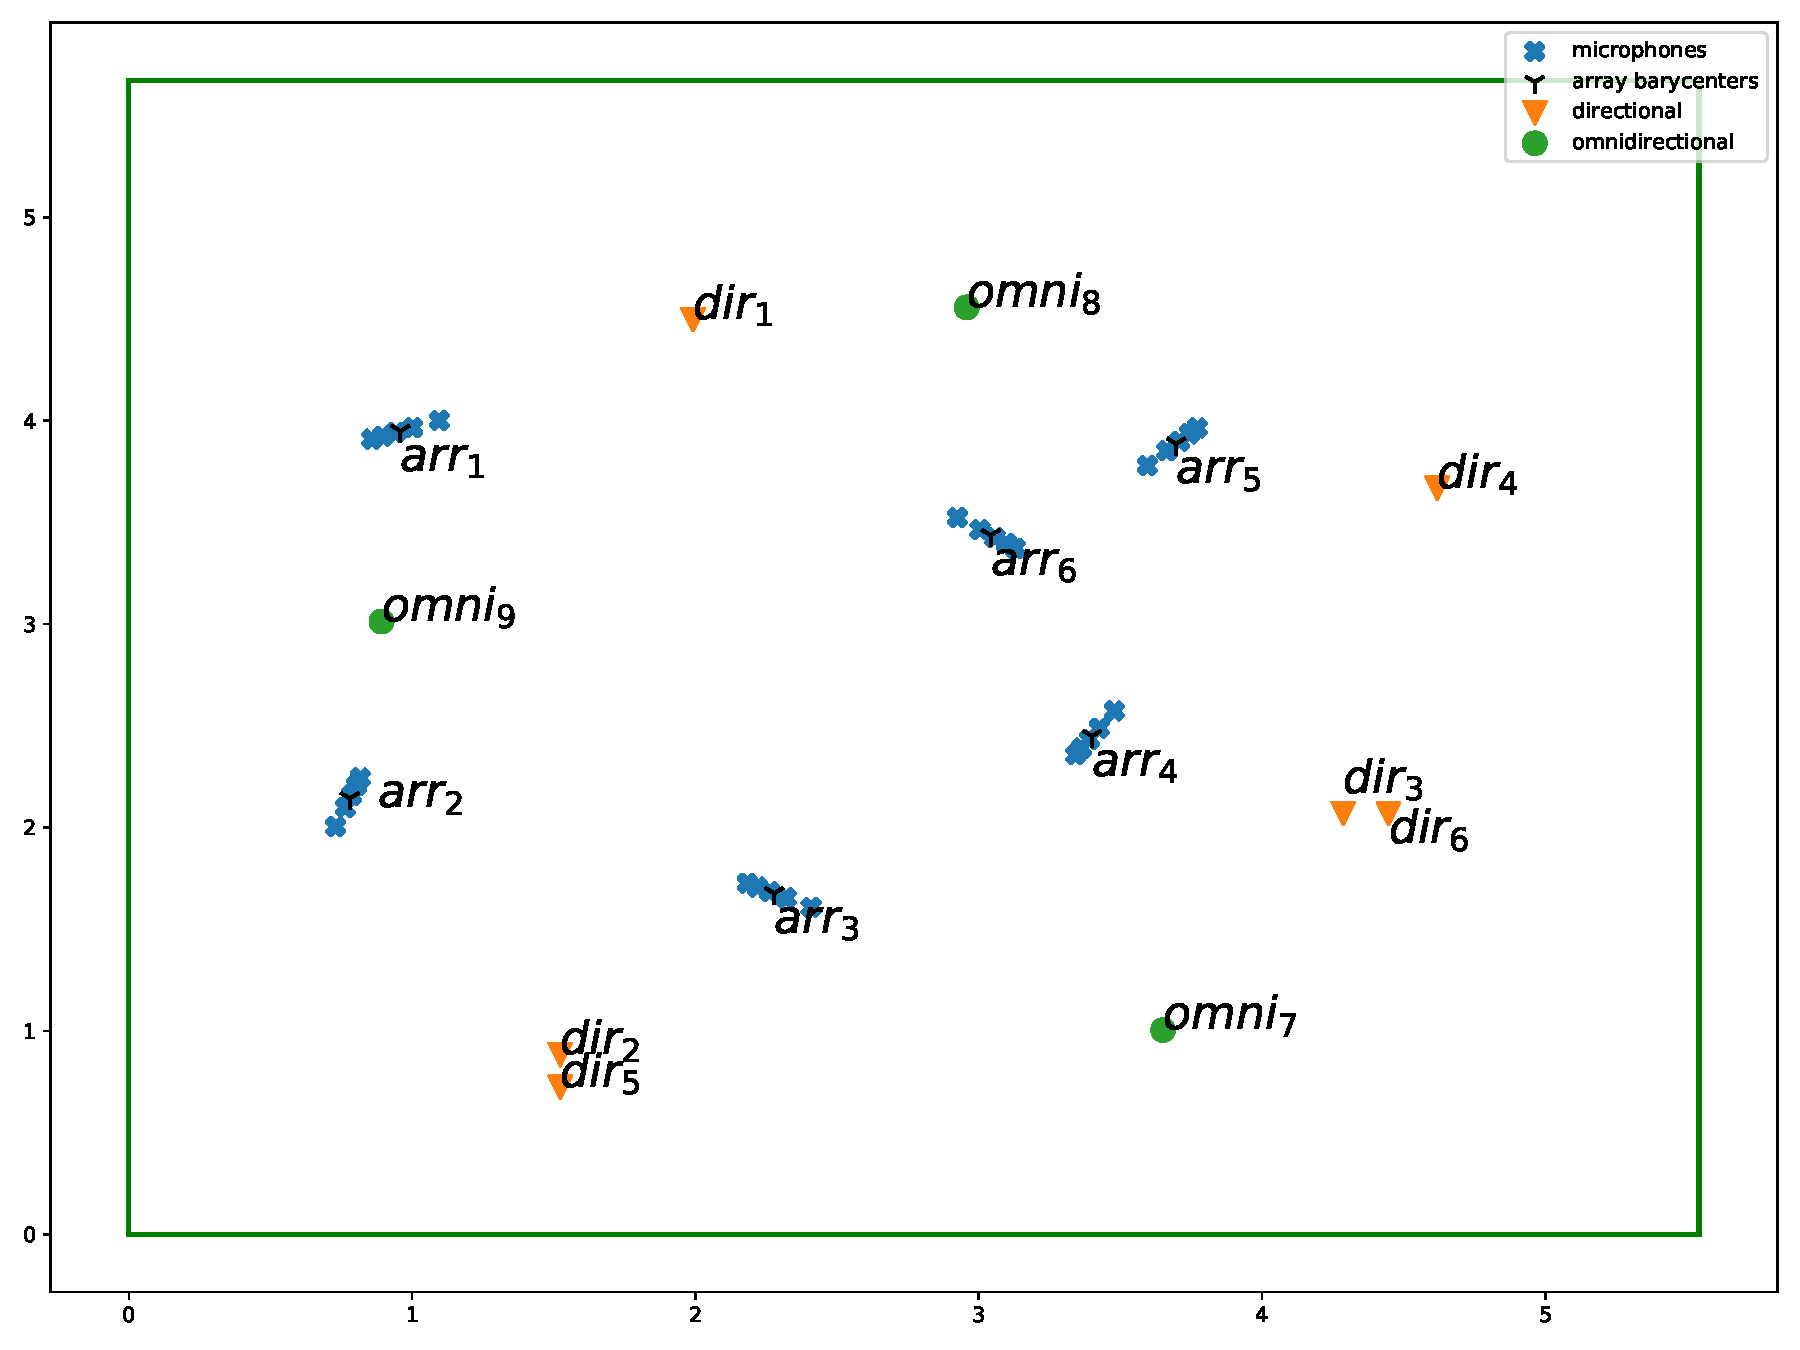
\includegraphics[width=\linewidth]{figures/dechorate/positioning2D_xy.pdf}
    \caption{Illustration of the recording setup - top view.}
    \label{fig:2D}
\end{figure}

% \begin{figure}[h]
%     \hfill
%     \subfigure{
%         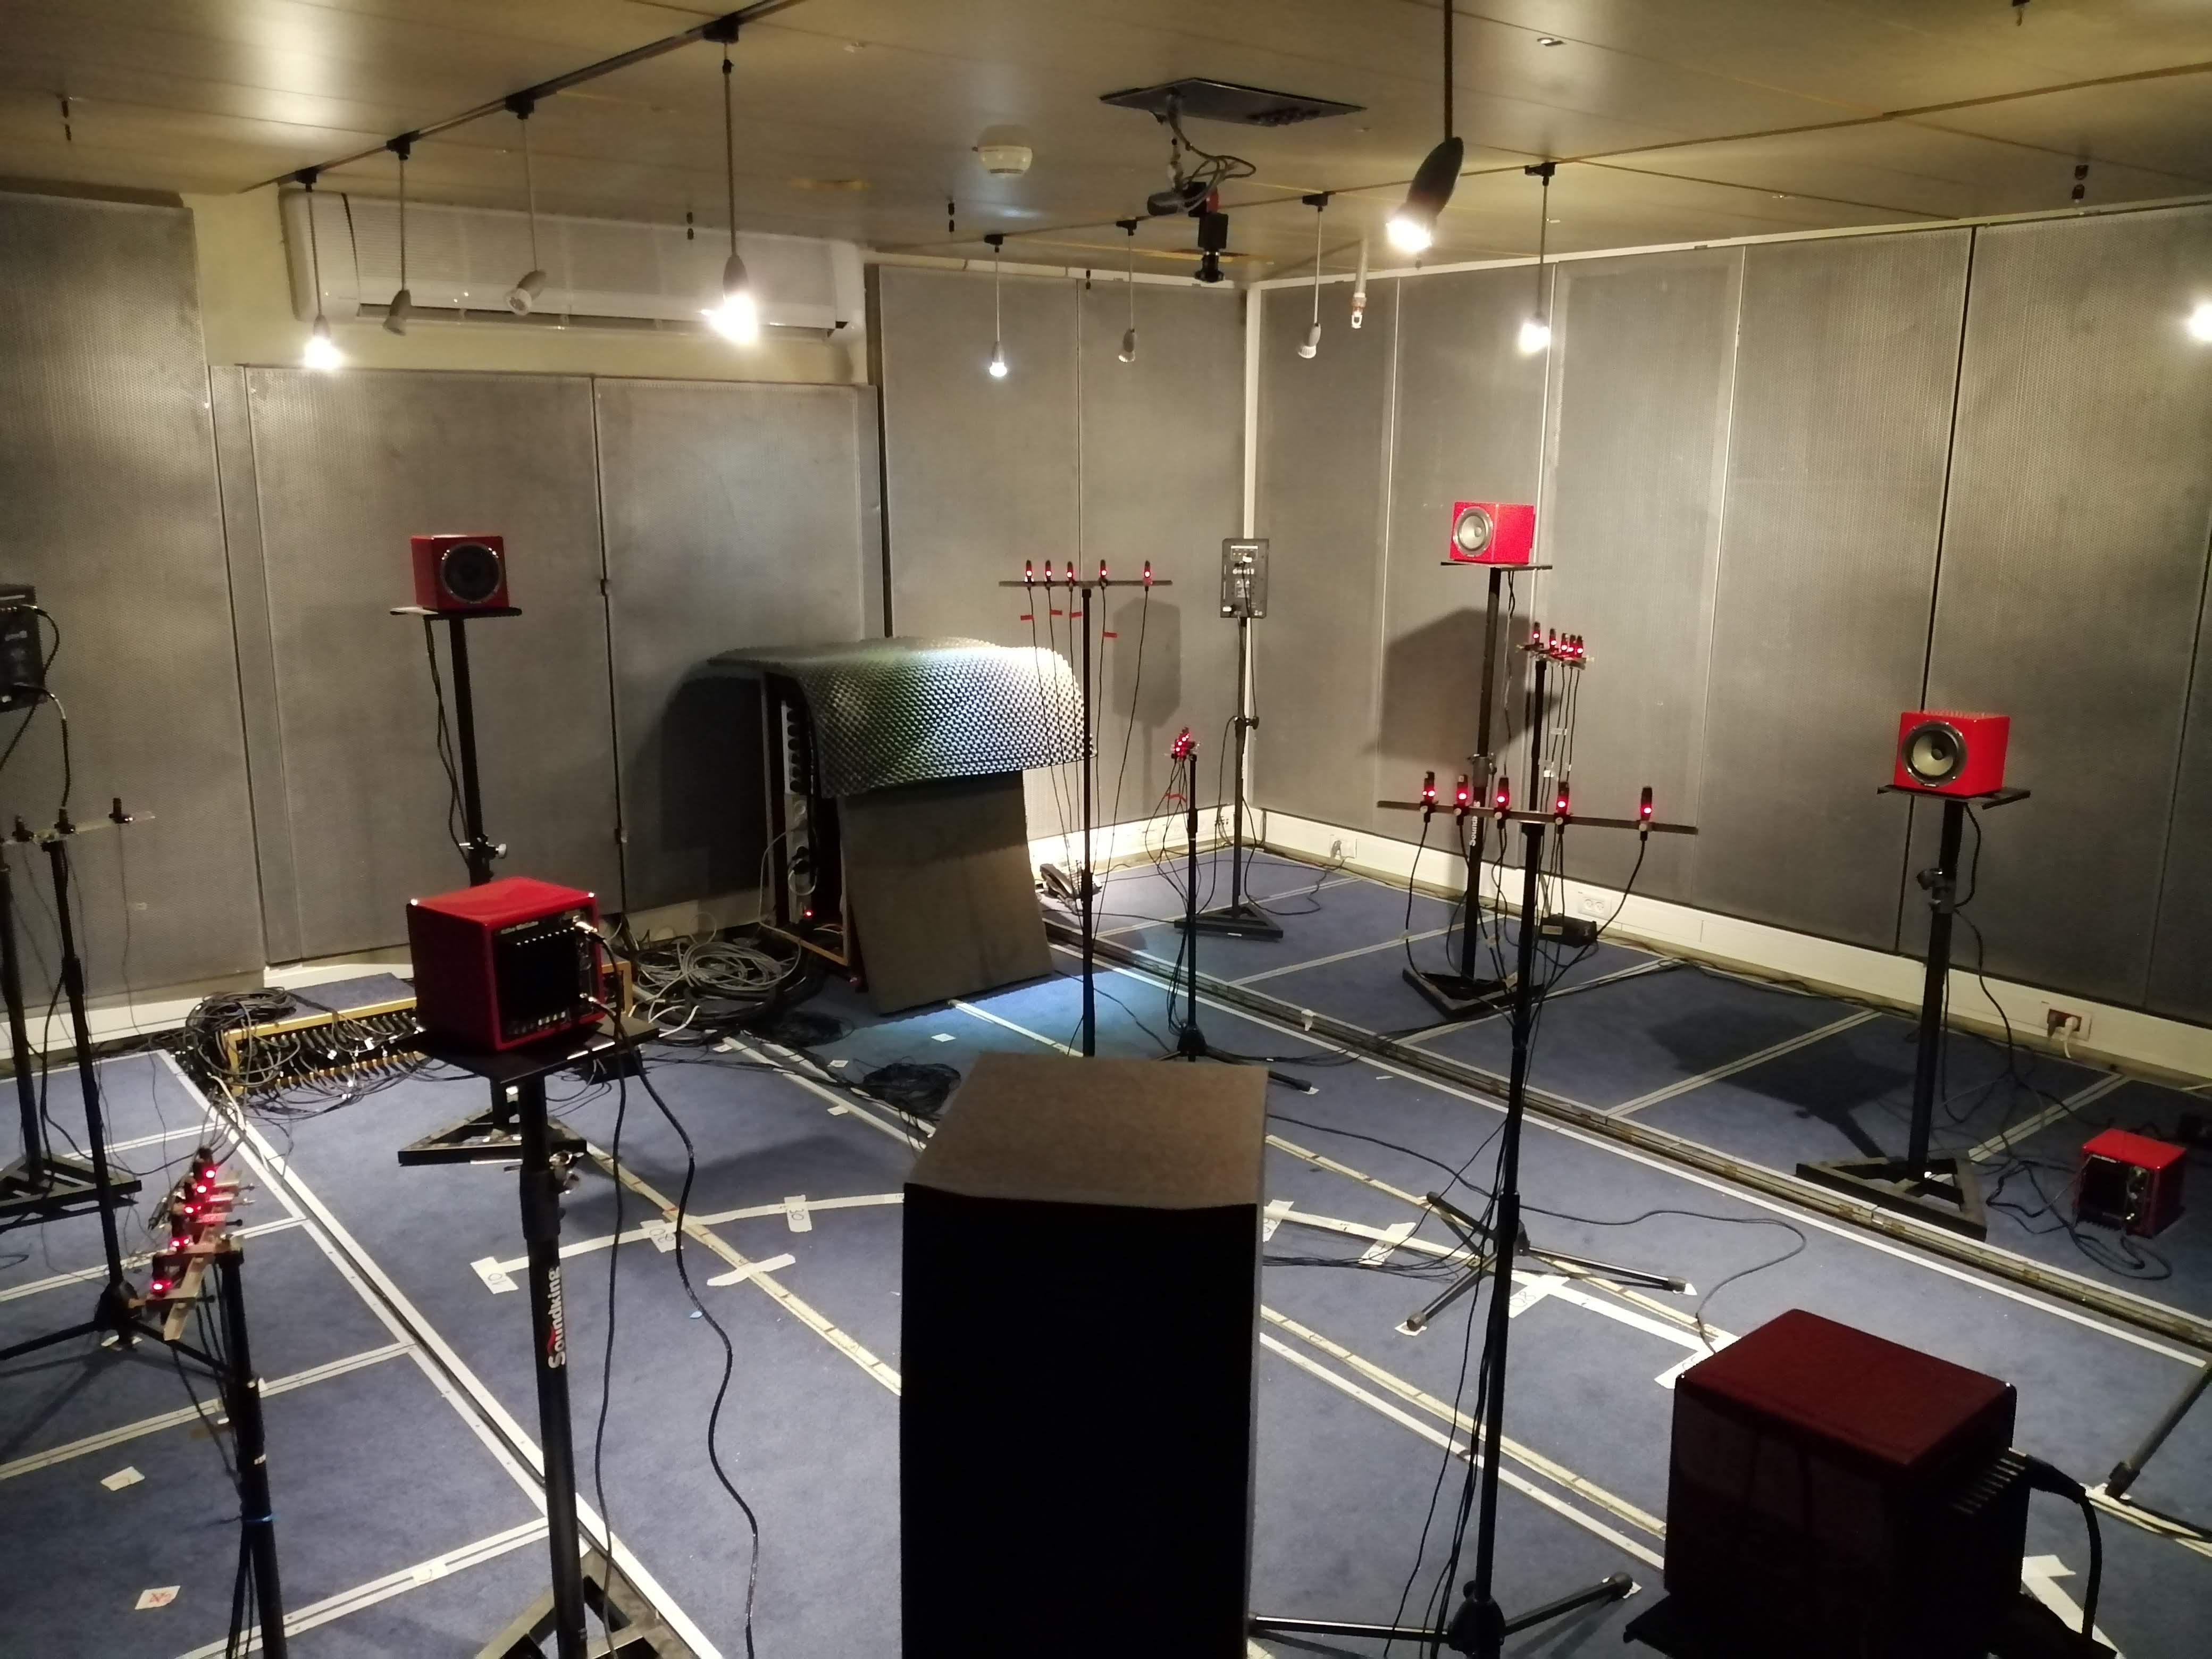
\includegraphics[width=0.325\textwidth]{
%             figures/dechorate/recording_setup}}
%     \hfill
%     \subfigure{
%         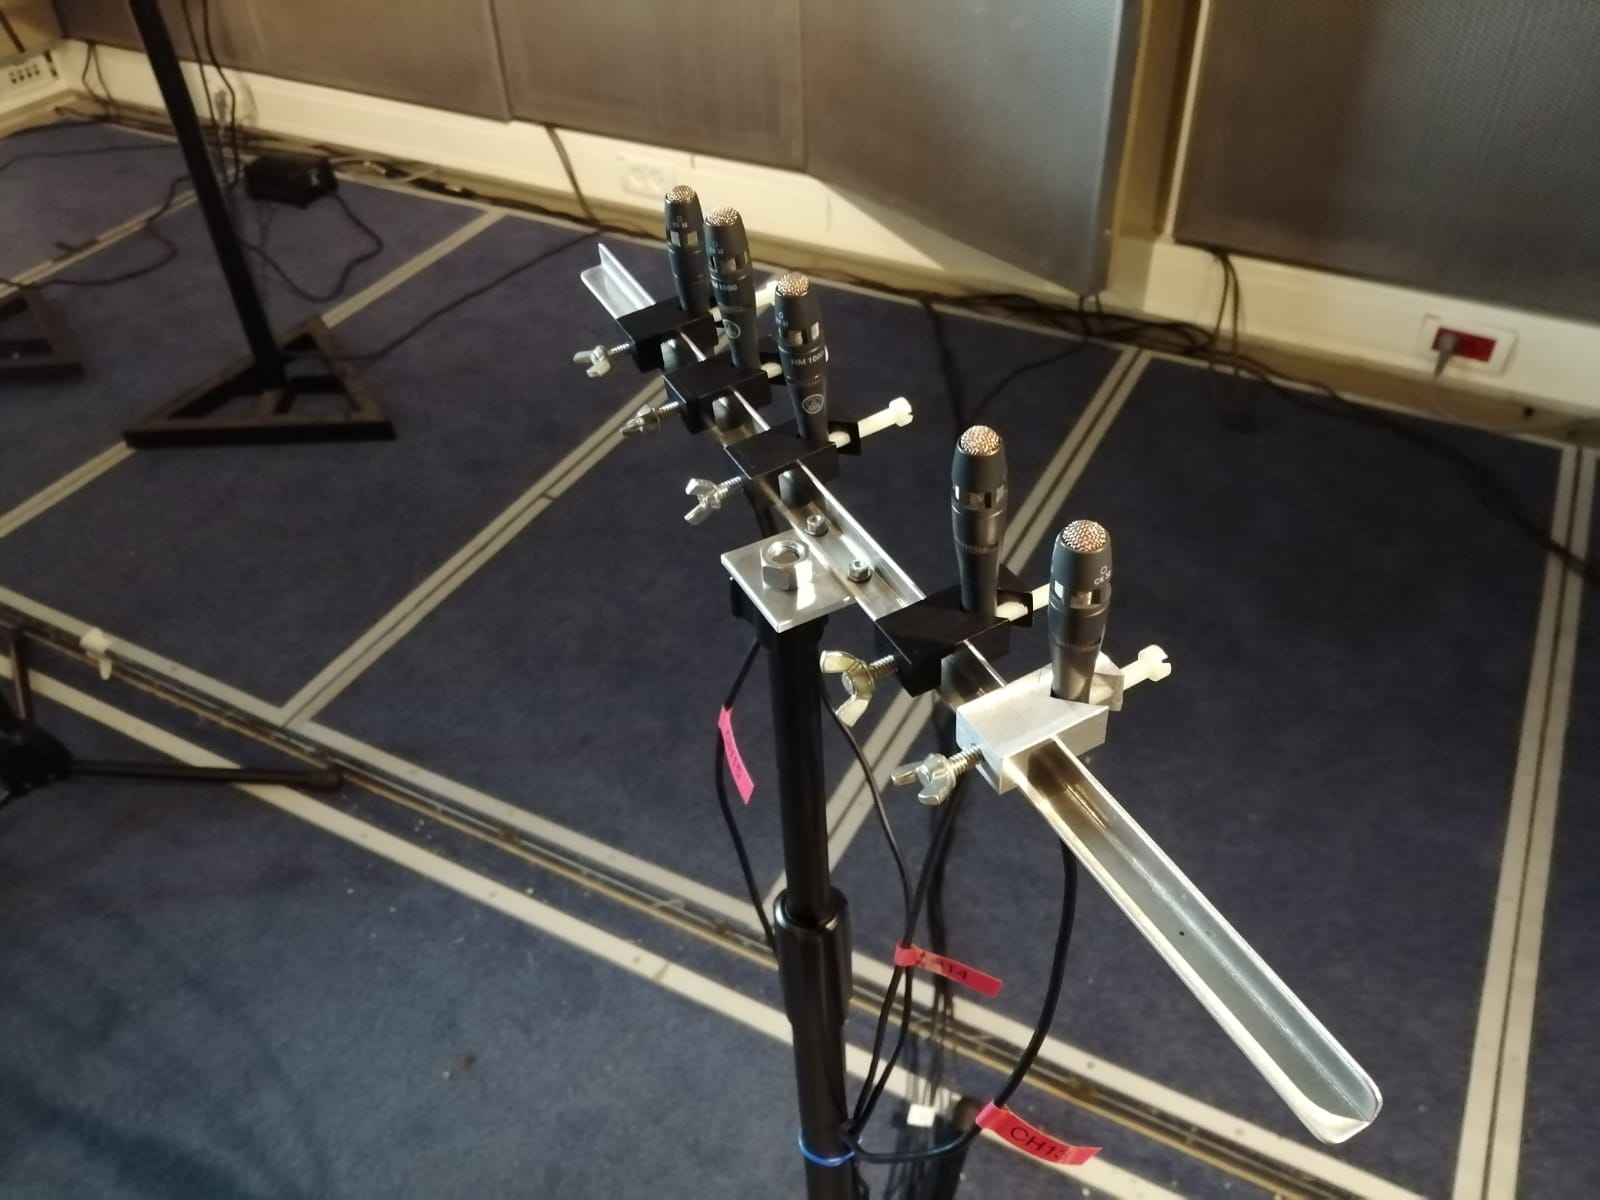
\includegraphics[width=0.325\textwidth]{
%             figures/dechorate/mic}}
%     \hfill
%     \subfigure{
%         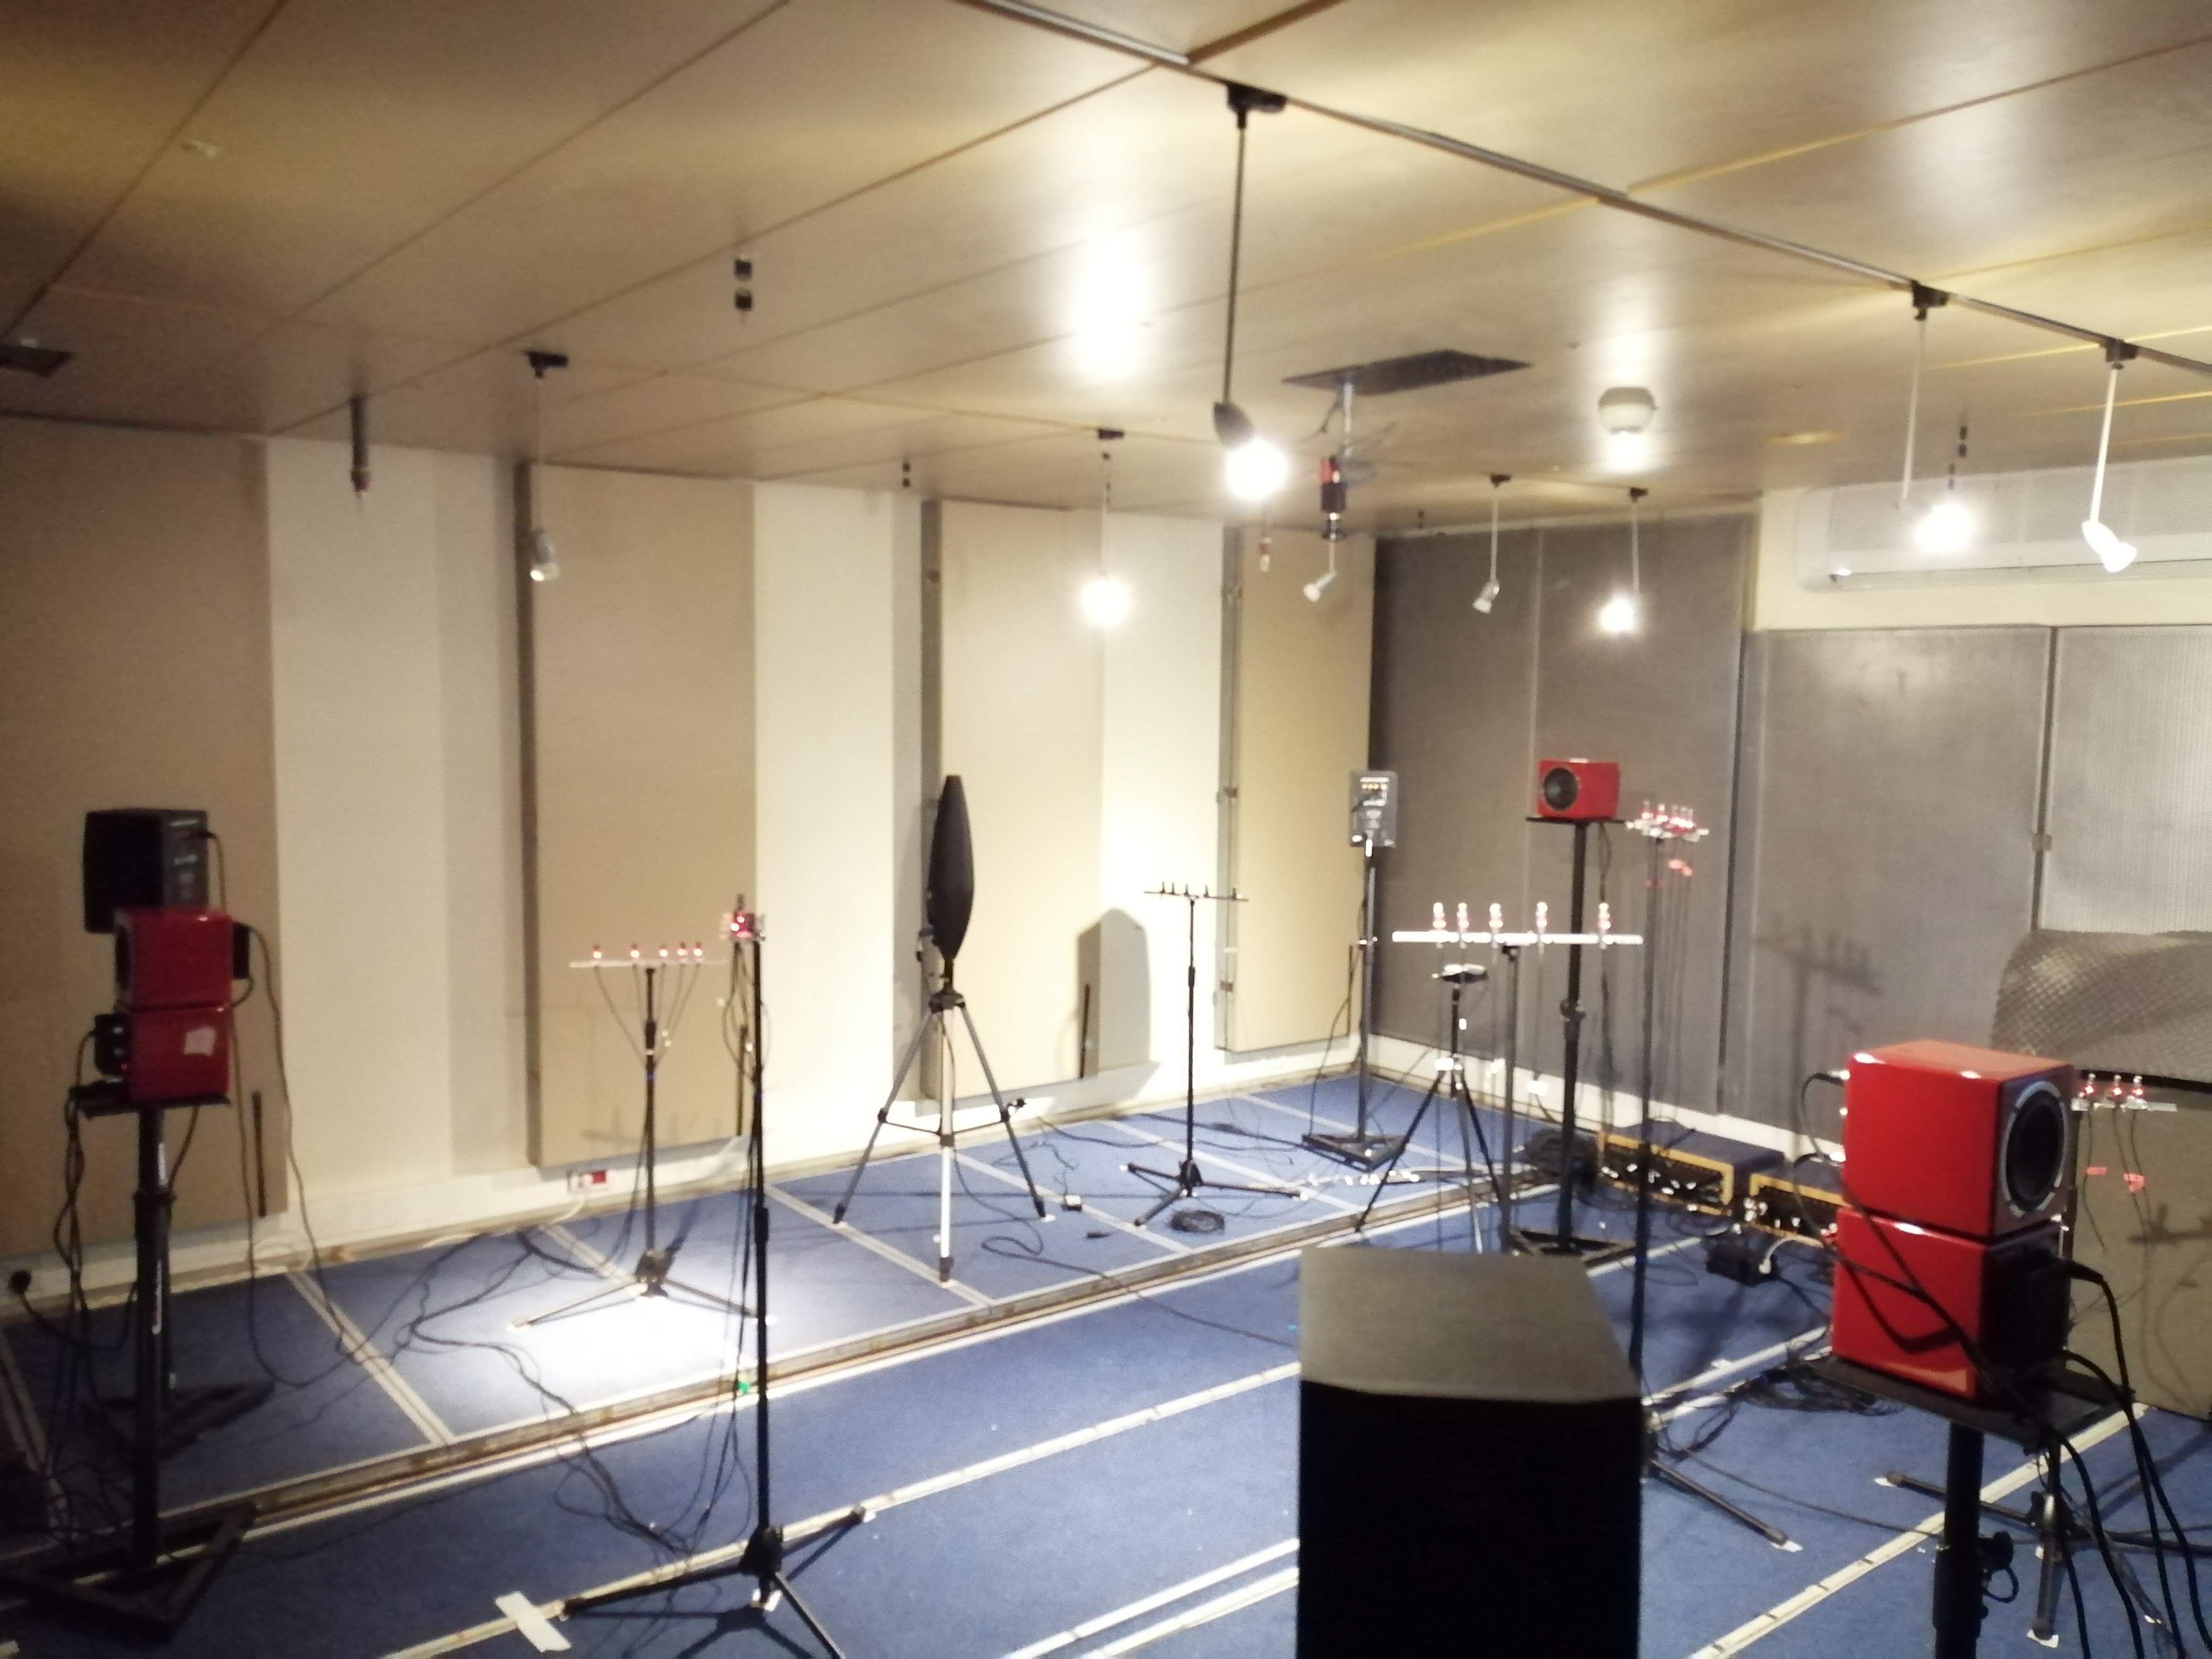
\includegraphics[width=0.325\textwidth]{
%             figures/dechorate/panels}}
%     \caption{Picture of the acoustic lab. From left to right: the overall setup, one microphone array, the setup with revolved panels.}
%     \label{fig:setut}
% \end{figure}

\subsection{Realization}
The main feature of this room is the capability to change the acoustic profile of the each of its facet by flipping double-sided panels with one reflective and one absorbing face. This allows to achieve precise values of $\RT$ that ranges from $0.1$ to almost $1$ second. In this dataset the panels of the floor were kept always absorbent.

Two types of sessions were considered, namely, \textit{one-hot} and \textit{incremental}. For the first type, a single facet was placed in reflective mode while all the others were kept absorbent. For the second type, starting from fully-absorbent mode, facets were progressively switched to reflective one after the other until all but the floor are reflective, as shown in Table \ref{tab:wallcoding}.

\begin{tabular}{cc|cccccc}
\toprule
& Surfaces:                 & Floor                 & Ceiling               & West                  & South                 & East                  & North                 \\ \hline
\multicolumn{1}{c}{\multirow{5}{*}{\rotatebox{90}{one-hot}}} & $\mathtt{000000}$                   & \xmark & \xmark & \xmark & \xmark & \xmark & \xmark \\
& $\mathtt{010000}$                    & \xmark & \cmark & \xmark & \xmark & \xmark & \xmark \\
& $\mathtt{001000}$                    & \xmark & \xmark & \cmark & \xmark & \xmark & \xmark \\
& \multicolumn{1}{c|}{$\dots$}  & \multicolumn{6}{c}{$\dots$} \\
& $\mathtt{000001}$                    & \xmark & \xmark & \xmark & \xmark & \xmark & \cmark \\
\multicolumn{1}{c}{\multirow{4}{*}{\rotatebox{90}{incremental}}} & $\mathtt{011000}$                    & \xmark & \cmark & \cmark & \xmark & \xmark & \xmark \\
& $\mathtt{011100}$                    & \xmark & \cmark & \cmark & \cmark & \xmark & \xmark \\
& \multicolumn{1}{c|}{$\dots$} & \multicolumn{6}{c}{$\dots$}  \\
& $\mathtt{011111}$                    & \xmark & \cmark & \cmark & \cmark & \cmark & \cmark \\
\bottomrule
\end{tabular}



% \\One recording session with random fornitures inside, to simulate the a typical meeting room with chairs, tables. The $\RT$ is around .

For each room configuration and loudspeaker, three different excitation signals were played and recorded in sequence: chirps, white noise and speech utterances. The former consists in a repetition of 3 exponentially swept-frequency sine (ESS) signals of duration 10 seconds and frequency range from 100 Hz to 14 KHz interspersed with 2 seconds of silence. Such frequency range was chosen to match the characteristics of the loudspeakers. To prevent rapid phase changes and ``popping'' effects, the signals were linearly faded in and out over 0.2 seconds with a Tuckey taper window\sidenote{\url{https://github.com/maj4e/pyrirtool}}.
Secondly, 10 seconds bursts of white noise and 3 anechoic speech utterances from the Wall Street Journal dataset \cite{Paul1992design} were reproduced in the room. Through all the recordings, at least 40 dB of sound dynamic range was asserted and room temperature of $\ang{24} \pm \ang{0.5}$ and humidity of $80\%$ were registered. Moreover 1 minute of \textit{room tone} (silence) and 4 minutes of diffuse babble noise were recorded for each session. The latter was simulated by transmitting different chunks of the same single-channel babble noise recording from additional loudspeakers facing the four corners of the room.

All the microphone signals were synchronously acquired and digitally converted to 48 kHz with 32 bits/sample using the equipment listed in Table~\ref{tab:room_equipment}. The polarity of each microphone was registered by clapping a book in the middle of the room.

\subsection{RIRs estimation and annotation}\label{sec:annotation}
RIRs are estimated with the ESS technique \cite{Farina2007advancements}: the signal of a microphone recording an ESS source is deconvolved by division in the frequency domain. Notice that the Fourier transform of the ESS signal used at the denominator is available in closed form.

The objective of this database is to feature annotations in the ``geometrical space'', namely the microphone and source positions, \textit{fully consistent} with annotations in the ``signal space'', namely the echo timings within the RIRs. This results is achieved as follows:
\begin{enumerate}[label=(\roman*)]
\item \label{it:ips} First, a the ground truth positions of array and source centres are acquired via a Beacon indoor positioning system ($\bIPS$). This system consists in 4 stationary bases positioned at the corners of the ceiling and a moving probe used for measurements which can be located within errors of $\pm2$~cm.

\item \label{it:not}  The estimated RIRs are superimposed on synthetic RIRs computed with the ISM from the geometry obtained in the previous step. A Python GUI, available in the database package, was used to manually tune a peak finder and \textit{label} there echoes, that is annotate their positions and their correspondent wall.

\item \label{it:mds} By solving a ``simple'' multi-dimensional scaling (\MDS) problem \cite{dokmanic2015relax, Crocco2016, Plinge2016acoustic}, refined microphone and source positions were computed. The non-convexity of the problem was alleviated by using a good initialization (obtained at the previous step), by the high SNR of the measurements and, later, by including the additional image sources in the formulation. The prior information about the arrays' structures reduced the number of variables of the problem, corresponding to the 3D positions of the sources and of the arrays' barycenters in addition to the the arrays' tilt on the azimuthal plane.

\item \label{it:lat} By employing a multilateration algorithm  \cite{Beck2008ExactProblems}, where the position of one microphone per array served as anchors and the TOAs are converted into distances, it was possible to localize the image sources along side with the real one as depicted in Figure~\ref{fig:wall_rec}.
\end{enumerate}

Knowing the geometry of the recording room, we were able to manually label the echoes by iterating through steps \ref{it:not}, \ref{it:mds} and \ref{it:lat}.
The final geometrical and signal annotation was chosen as a compromise between the $\bIPS$ measurements and the $\MDS$ output. While the formers are noisy but consistent with the scene's geometry, the latters match the TOAs but not necessarily the physical world. In particular, the geometrical ambiguities such as global rotation, translation and up-down ambiguities were observed. Instead of manually correcting this error, we modified the original problem from using only the direct distances ($\dMDS$) to considering the  image sources' TOA of the ceiling in the cost function ($\dcMDS$). Table~\ref{tab:res_mds} shows numerically the \textit{mismatch} (in cm) between the geometric space (defined by the $\bIPS$ measurements) and the signal space (the one defined by the echo timings, converted in cm).  To better quantify it, we introduce here the \textit{goodness of match} (GoM): it measures the fraction of (first-order) echo timings annotated on the RIRs matching the annotation produced by the geometry within a threshold. Including the ceiling information, $\MDS$ produces a geometrical configuration which has a small mismatch (0.41 cm in average) in both the signal \textit{and} geometric spaces with $98.1\%$ of matching first order echoes within 1 ms window. Nevertheless, it is interesting to see that already the $\bIPS$ measurements produces a good but less precise annotation.

\begin{tabular}{lllll}
\toprule
& Metrics        & $\bIPS$               & $\dMDS$          & $\dcMDS$          \\
\midrule
\multicolumn{1}{c}{\multirow{2}{*}{\rotatebox{90}{\footnotesize Geom.}}}
&   Max.             & -            & $6.1$         & $1.07$        \\
&   Avg.$\pm$Std.    & -            & $1.8\pm1.4$    & $0.39\pm0.2$  \\
% \rule{0pt}{0.1em}\\
\midrule
\multicolumn{1}{c}{\multirow{2}{*}{\rotatebox{90}{\footnotesize Signal}}}
&   Max.          & $5.86$         & $1.20$         & $1.86$       \\
&   Avg.$\pm$Std. & $1.85\pm 1.5$  & $0.16\pm0.2$   & $0.41\pm0.3$ \\
% \rule{0pt}{0.1em}\\
\midrule
\multicolumn{1}{c}{\multirow{3}{*}{\rotatebox{90}{\footnotesize Mismatch}}}
&  GoM (1.0 ms)   & $97.9 \%$      & $93.4 \%$      & $98.1 \%$ \\
&  GoM (0.1 ms)   & $26.6 \%$      & $44.8 \%$      & $53.1 \%$ \\
&  GoM (0.05 ms)  & $12.5 \%$      & $14.4 \%$      & $30.2 \%$ \\
\bottomrule
\end{tabular}


Finally, we want to mention that the following tools and techniques were found helpful in annotating the echoes:

\newthought{The \texttt{skyline} visualization} consists in presenting multiple RIRs as an image, such that the wavefronts corresponding to echoes can be highlighted \cite{Baba2018b}. More precisely, it is the visualization of the $L \times N$ matrix $\mathbf{H}$ created by stacking column-wise $N$ normalized echograms\sidenote{The echogram is defined either as the absolute value or as the squared value of the RIRs.}, that is $\mathbf{H}_{l, n} =\bar{\eta}_{n}(l) = \kvbar{h_{n}(l)}/\max{\kvbar{h_{n}(l)}}$, where $l = 0, \dots, L-1$ is  the sample index and $n$ is an arbitrary indexing of the all microphones for a fix room configuration. 4 RIR $\mathtt{skyline}$s for 4 directional sources for the full reflective scenario are shown in Figure~\ref{fig:skyline}, stacked horizontally, preserving the order of microphones within the arrays. Thus, the reader can notice several clusters of 5 adjacent points of similar color (intensity) corresponding to the arrivals at the array's sensors. Thanks to the usage of linear arrays, this visualization allowed us to identify both TOAs and their labeling.

\begin{figure}[h]
    \centering
    \begin{overpic}[width=\linewidth]{figures/dechorate/labeling_tool.pdf}
    \put (2,62) {\footnotesize a)}
    \put (52,62) {\footnotesize b)}
    \put (2,31) {\footnotesize c)}
    \put (52,31) {\footnotesize d)}
    \end{overpic}

    \caption{Detail of the GUI used to manually annotate the RIRs. For a given source and microphone, a) and b) shows 2 RIR for 2 different room walls configuration (blue and orange) before and after the direct path deconvolution respectively. c) shows the results of the peak finder of the equalized RIR and d) is a zoom on the RIR Skyline (see Fig.~\ref{fig:skyline}).}
    \label{fig:labelling_tools}
\end{figure}


\begin{figure}
    \centering
    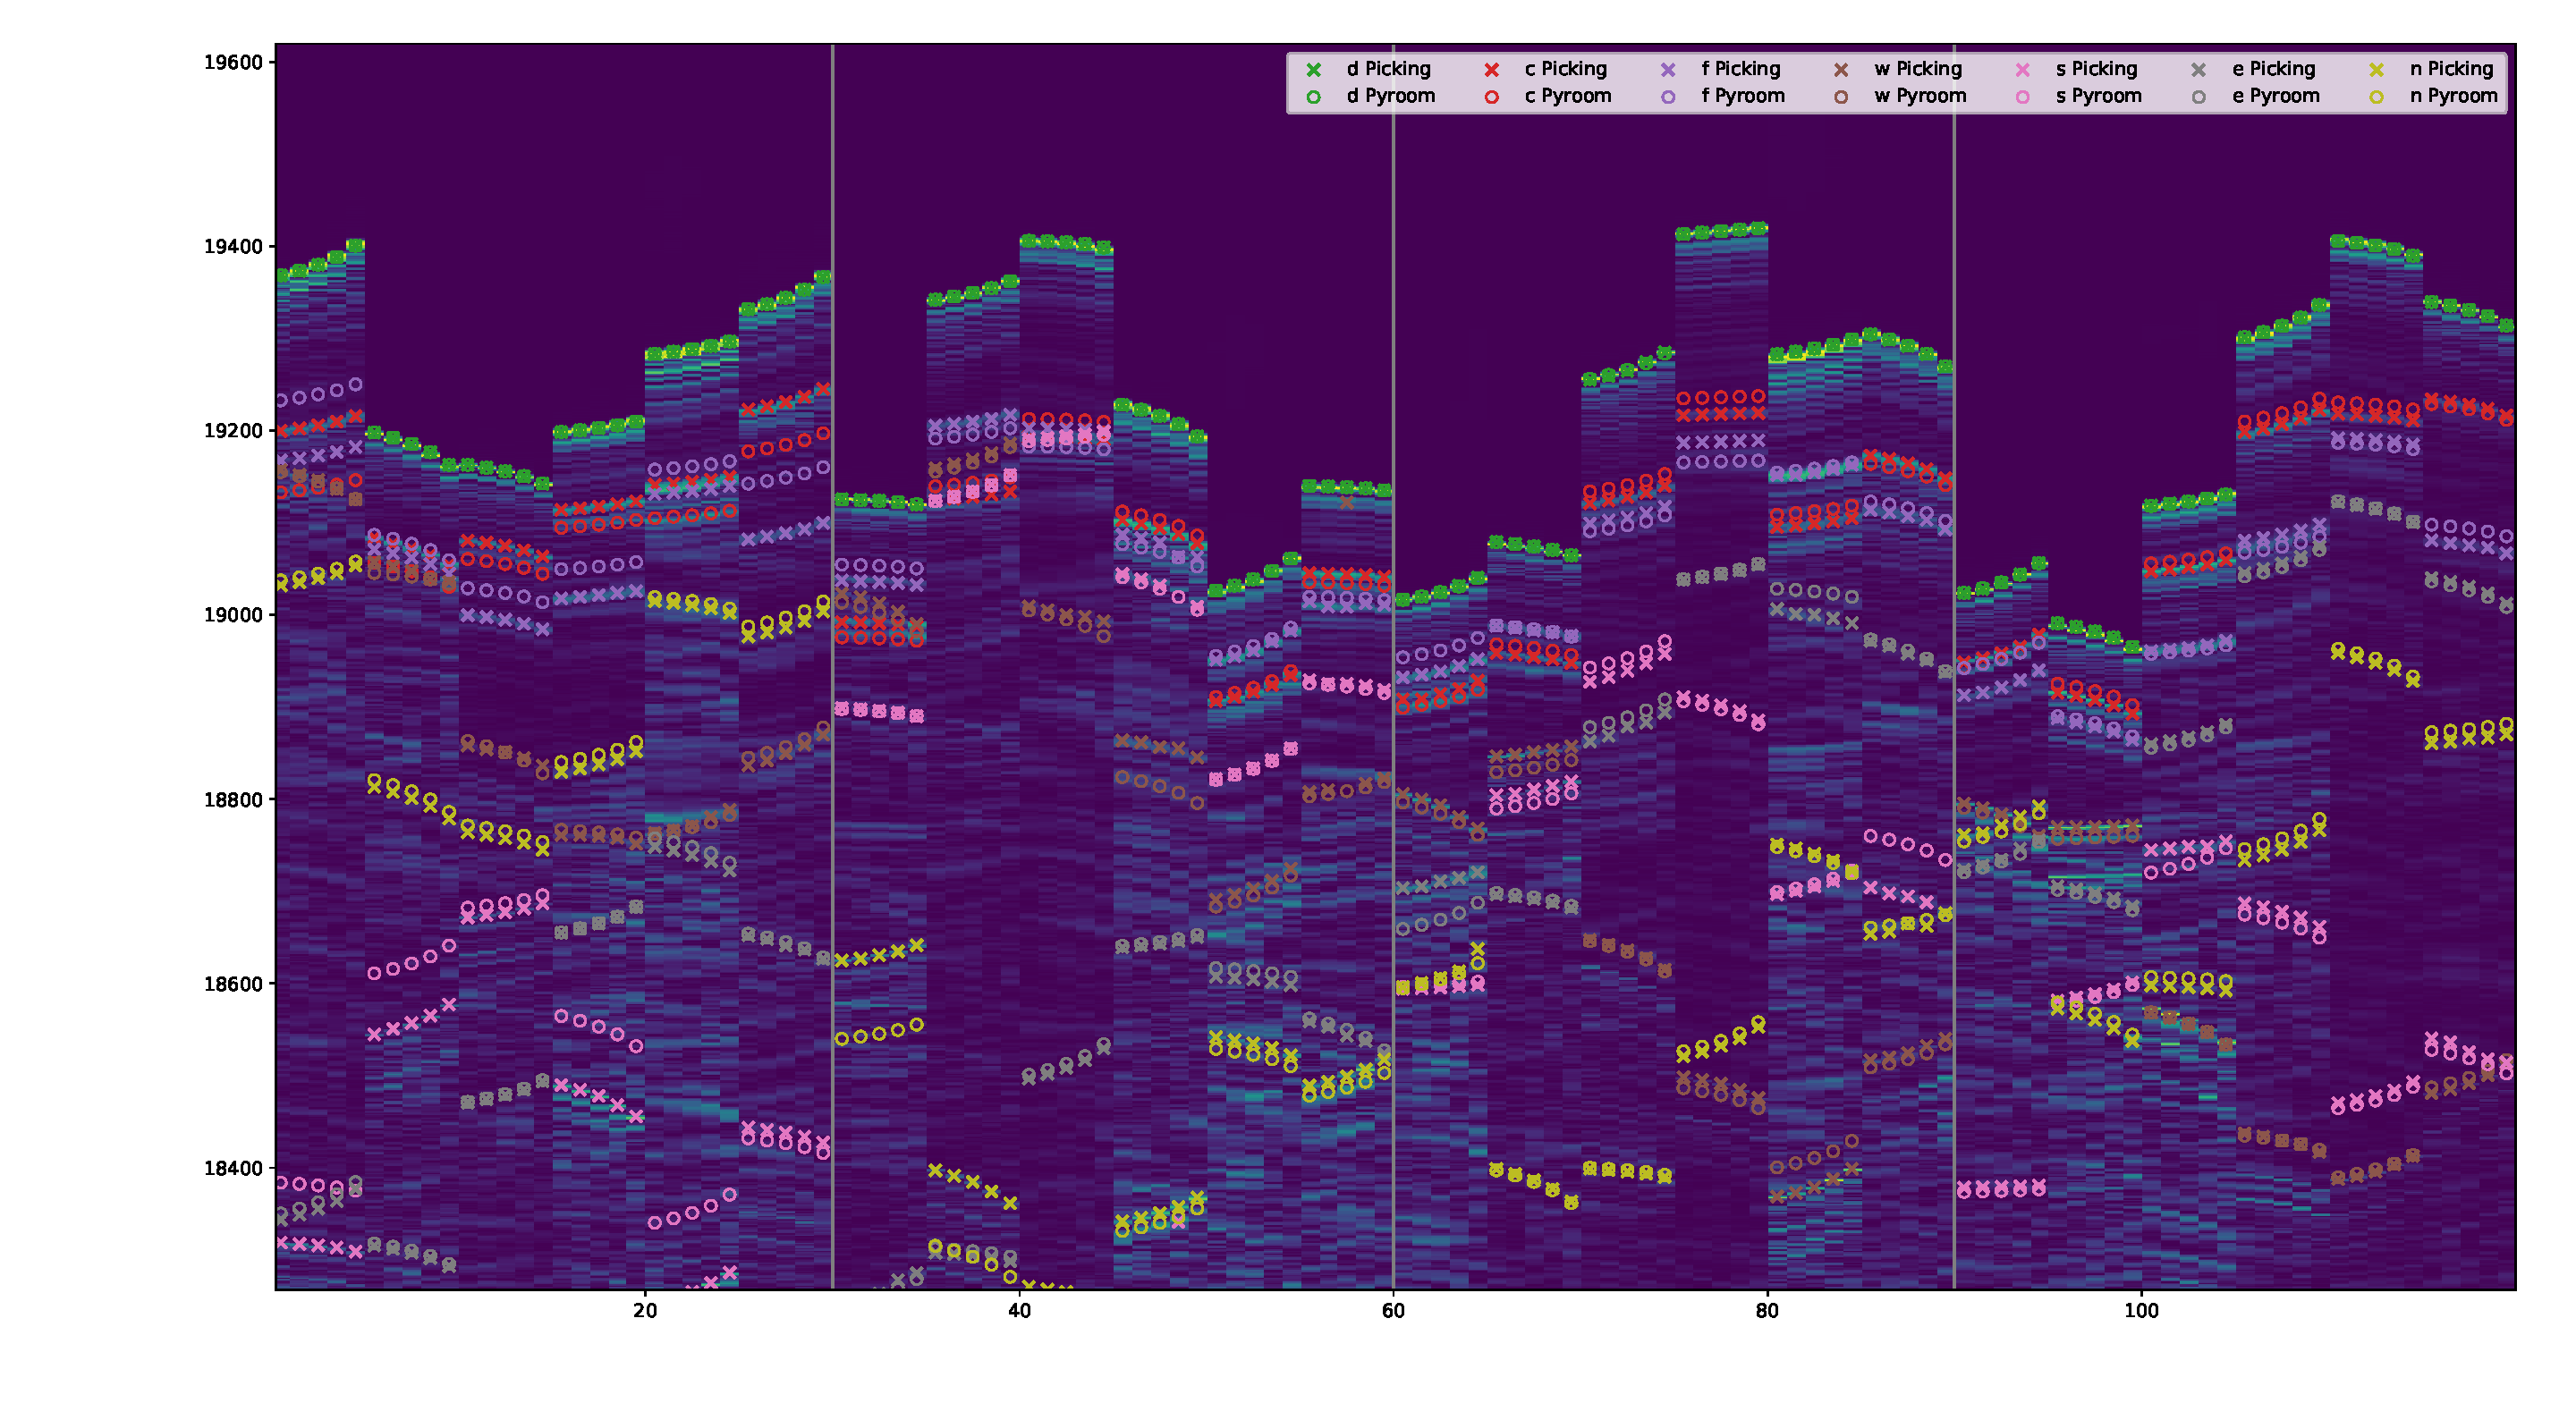
\includegraphics[width=\linewidth]{figures/dechorate/rir_skyline_final_mod4paper.pdf}
    \caption{RIR $\mathtt{Skyline}$ annotated with observed peaks ($\times$) together with their geometrically-expected position ($\circ{}$) computed with Pyroomacoustic simulator. As specified in the legend, different colors are used to indicate the room facets responsible for the reflection: direct path ($\mathtt{d}$), ceiling ($\mathtt{c}$), floor ($\mathtt{f}$), west wall ($\mathtt{w}$), $\dots$, north wall ($\mathtt{n}$).}
    \label{fig:skyline}
\end{figure}

\newthought{Direct Path Deconvolution} (or equalization) was used for compensating the frequency response of the source loudspeaker and microphone \cite{antonacci2012inference, Eaton2016estimation}. In particular, the direct path of the RIR was manually isolated and used as an equalization filter for enhancing early reflections from their superimposition and from background noise before proceed with peak picking. Each RIR was equalized with its relative direct path. As depicted in Figure~\ref{fig:labelling_tools}, in some situation this process was necessary for correctly identifying the underlying TOAs' peaks.

\newthought{Different Wall Combinations} for the same geometry influenced the peaks' predominance in the RIR, hence hence facilitating its echo annotation. An example of RIRs corresponding to 2 different surface configurations is shown in Figure~\ref{fig:labelling_tools}: the reader can notice how the peak prominence change for the different configurations.

\newthought{The Interpolation-based Peak Finder\sidenote{\url{https://bitbucket.org/lucashnegri/peakutils/}}} was used on the normalized echograms $\bar{\eta}_{n}(l)$ to sightly compensate the sampling process. In~\cite{remaggi2017acoustic} a method that automatically extract peaks in RIRs is proposed. However, in practice, the manual peak finding was found easier and more robust.

\subsection{Limitations of current annotation}
As stated in \cite{Defrance2008finding}, we want to emphasize that annotating the correct TOAs of echoes and even the direct path in ``clean'' real RIRs is far from straightforward. The peaks can be blurred out by the loudspeaker characteristics or the concurrency of multiple reflections. However as showed in Figure~\ref{fig:skyline}, the proposed annotation was found to be sufficiently consistent both in the geometric and the echo in the echo space. Thus, no further refinement was done. This database can be used as a first basis to develop better AER methods which could be used to iteratively improve the annotation, for instance including  2$^\text{nd}$ order reflections.

\subsection{The dEchorate package}
The dataset comes with both data and code to parse and process them. The data are presented in 2 modalities: the $\mathtt{raw}$ data, that is, the collection of recorded wave files, are organized in folders and can be retrieved by querying a simple database table; the $\mathtt{processed}$ data, which comprise the estimated RIRs and the geometrical and signal annotations, are organized in tensors directly importable in Matlab or Python (\textit{e.g.} all the RIRs are stored in a tensor of dimension $L \times I \times J \times D$, respectively corresponding to the RIR length in samples, the number of microphones, of sources and of room configurations).
\\Together with the data a Python package is available at the same website. This includes wrappers, GUI, examples as well as the code to reproduce this paper.
In particular, all the scripts used for estimating the RIRs and annotating them are available and can be used to further improve and enrich the annotation or as baselines for future works.

\begin{figure}
    \centering
    
\includegraphics[width=\linewidth]{figures/dechorate/database.png}
    \caption{Sample view of the database table to retrieve the raw wave file and its attributes.}
    \label{fig:dataset}
\end{figure}

\section{Using the Data}
In this section we exemplify the utilization of the database considering three possible use-cases: acoustic echo estimation, echo-aware beamforming and room geometry estimation.

\subsection{Acoustic Echo Estimation}
\textit{Work in progress:
Use BSN, Crocco and BLASTER for echo acoustic echo retrieval.
\\Data: Sym/Real on Dirac/Noise/Speech}


\subsection{Echo-aware Beamforming}

\begin{figure}[h]
    \centering
    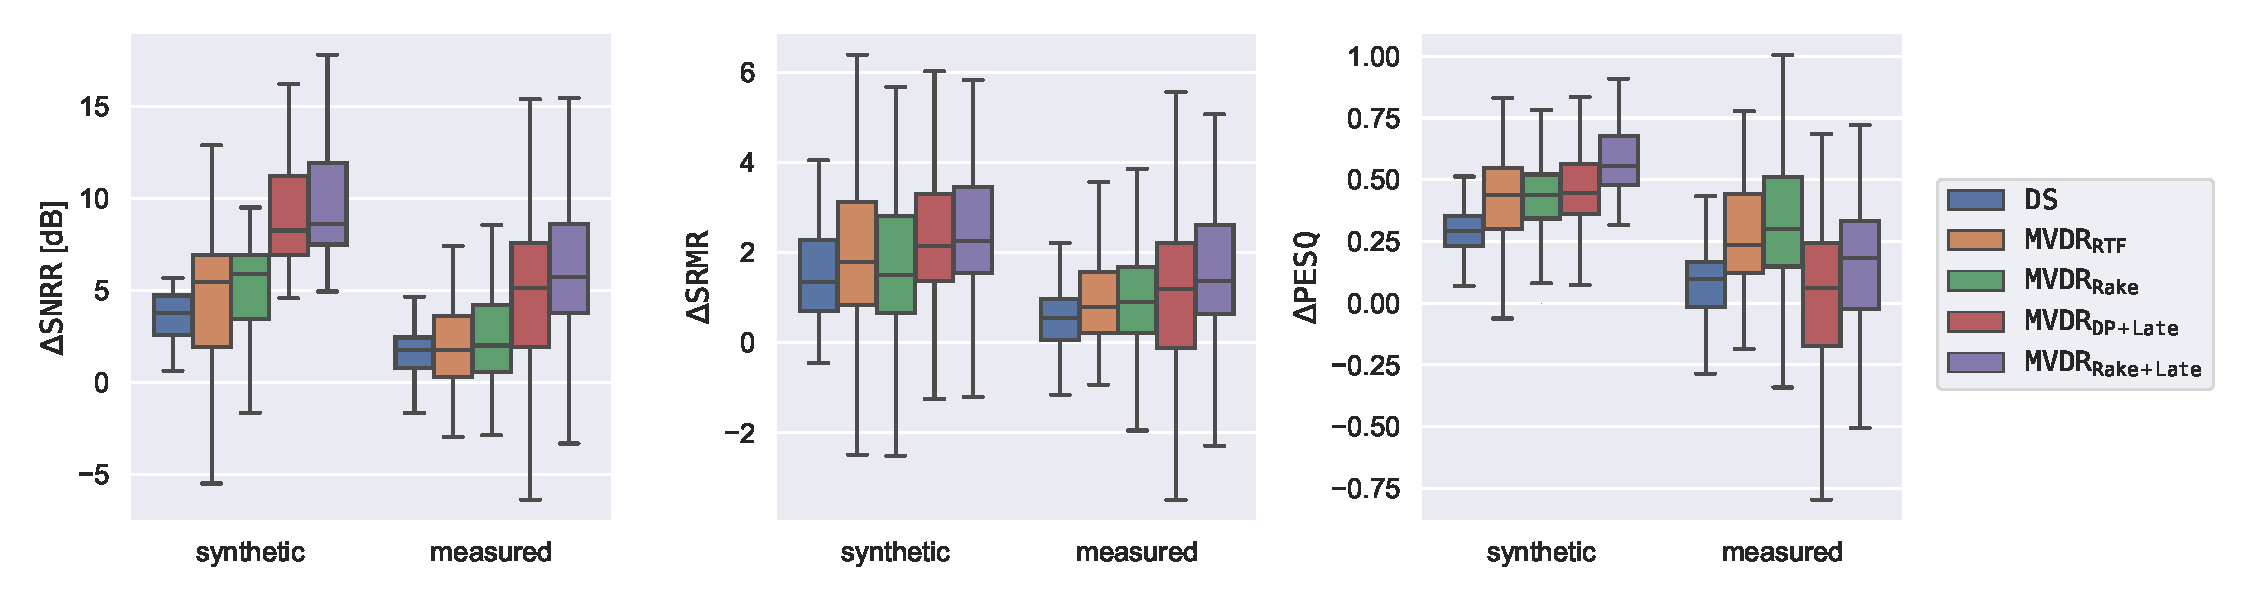
\includegraphics[trim={0 10 10 0},clip,width=\linewidth]
    {figures/dechorate/kowalkzy_results_boxplot.pdf}
    \caption{
    Comparison of echo-aware beamforming for the room configuration $\mathtt{011111}$ ($\RT \approx 600 $ ms) on measured and synthetic data  for all combinations of source-array positions in the \dEchorate{} dataset.}
    \label{fig:pesq}
\end{figure}

As mentioned, the knowledge of early echoes should boost spatial filtering performances. However the perfect knowledge of such elements are of difficult estimation. To investigate this, we compare two types of spatial filters on both synthetic and measured data: echo-agnostic and echo-aware beamformers.
\\The formers do not need any echo-estimation step: they either ignore their contributions, such in the direct-path delay-and-sum beamformer ($\DS$)~\cite{VanTrees2004Optimum}, or they consider coupling filters between pairs of microphones, called Relative Transfer Functions (RTFs)~\cite{Gannot2001signal}\footnote{Note that, as opposed to AER, estimating the RTF is a non-blind problem.}.
The RTFs can be naturally incorporated in powerful beamforming algorithms achieving speech dereverberation and noise reduction in static~\cite{Schwartz2014multi}
and dynamic scenarios~\cite{Kodrasi2017evd}.
In this work, generalized eigenvector decomposition (GEVD) was used for the RTFs estimation~\cite{doclo2003robust}.
\\Echo-aware beamformers fall in the category of \textit{rake receivers}, borrowing the idea from telecommunication where an antenna rakes (\textit{i.e.} combines) coherent signals arriving from different propagation paths.
In particular, they consider ``partial steering vectors'' using known $R$ echoes' delays and attenuations~\cite{Jan1995matched}. This methods have been used for interfer and noise suppression in~\cite{Dockmanic2015raking} and for noise and reverberation reduction~\cite{Javed2016spherical, Kowalczyk2019raking}. Here we assume that echoes are known, computed from the geometry as in Section~\ref{sec:annotation}.

In addition to the standard $\DS$ design, we considered the minimum-variance-distrortionless-response design
echo-agnostic $\MVDR_\mathtt{RTF}$ build on RTFs as in~\cite{Schwartz2014multi} as echo-agnostic method, and the echo-aware beamformers $\MVDR_\mathtt{Rake}$~\cite{Dockmanic2015raking} and its extension for dereverberation, the $\MVDR_\mathtt{Rake+Late}$~\cite{Kowalczyk2019raking} considers the statistical contribution of the reverberation tail.

The performances of the different designs are compared for enhancing a target speech in 5-channel mixture (that is, one linear array used in the dataset) featuring high reverberation and diffuse babble noise, opportunely scaled to given signal-to-noise  ratio ($\SNR \in \kbrace{0, 10, 20}$).
Using the \dEchorate{} data, we considered the room configuration $\mathtt{011111}$ ($\RT \approx 600 $ ms) and all the possible combinations of target/array's positions. Both real and matching synthetic RIRs are used which are then convolved with anechoic speech from the WSJ corpus and corrupted by recorded diffuse noise.

The evaluation is conducted similarly to the one in~\cite{Kowalczyk2019raking}. We considered the following metrics: the signal-to-noise-plus-reverberation improvment (\DSNRR) in [dB] computed as difference between the input ($\mathtt{SNRR}$) at the reference microphone and the $\mathtt{SNRR}$ at the filter output; the speech-to-reverberation-energy-modulation ratio improvement (\DSRMR)\cite{falk2010non} as measure of dereverberation; and the perceptual quality of the signal is evaluated using the PESQ score.
As target signal, the clean signal convolved with the early part of the RIR (up to the $R$-th echo) is considered.
\\Numerical results are reported in Figure~\ref{fig:pesq}.
The simple $\DS$ beamformer is outperformed by the other filters, since more information is used to reduce noise and late reverberation.
When using synthetic data, the know echoes perfectly match numerically the components in the simulated RIRs. In this ideal scenario, one can see that the more information used the better the performances: RTF- and Rake- beamformers outperform the simple $\DS$ design; and including the late reverberation statistics boosts considerably all the performances.
Interestingly RTF-based design performs similarly to the Rake-one. This can be explained by the fact that GEVD method tends to robustly consider the stronger and more stable components of the RTFs, which in reverberant and noisy static scenario's are similar to the earlier portion of the RIRs.
\\When it comes to measured RIRs, the little errors in echo estimation, due to calibration mismatch, lead to a drop in the performances. This is even more clear when considering the $\dPESQ$ metrics, as it accounts also for artifacts. Here the echo-agnostic $\MVDR_\mathtt{RTF}$ outperform the other methods.


\begin{tabular}{c|cc|cc|cc|cc}
\toprule
source id &	1	& &	2	& &	3	& &	4 &	\\
wall &	DE&	AE&	DE&	AE&	DE&	AE&	DE&	AE\\
\hline
west &	0.74	& $\ang{8.99}$      & 4.59	& $\ang{8.32}$  & 5.89	& $\ang{5.75}$	& $\mathbf{0.05}$    & $\mathbf{\ang{2.40}}$\\
east &	$\mathbf{0.81}$	& $\mathbf{\ang{0.08}}$      & 0.9	& $\ang{0.50}$	&$\mathit{69.51}$	& $\mathit{\ang{55.70}}$	& 0.31    & $\ang{0.21}$\\
south&	3.94	&$\ang{16.08}$      & $\mathbf{0.18}$	& $\ang{1.77}$	&$\mathit{14.37}$ & $\mathit{\ang{18.55}}$	& 0.82    & $\mathbf{\ang{1.65}}$\\
north&	1.34	& $\ang{0.76}$	    & 1.40	& $\ang{8.94}$	& $\mathbf{0.63}$	& $\mathbf{\ang{0.17}}$	& 2.08    & $\ang{1.38}$\\
floor&	$\mathbf{5.19}$	& $\mathbf{\ang{1.76}}$	    & 7.27	& $\ang{2.66}$	& 7.11	& $\ang{2.02}$	& 5.22    & $\ang{1.90}$\\
ceiling&1.16	& $\ang{0.28}$	    & 0.67	& $\ang{0.76}$	& $\mathbf{0.24}$	& $\ang{1.16}$	& $0.48$    & $\mathbf{\ang{0.26}}$\\

\bottomrule
\end{tabular}

\subsection{Room Geometry Estimation}
The shape of a convex room can be estimated knowing the positions of first-order image sources. Several methods have been proposed which take into account different levels of prior information and noise (see~\cite{remaggi2017acoustic, Crocco2018room} for a review). Nonetheless, when the echoes' TOA and their labeling are known for 4 non-coplanar microphones, one can perform this task using simple geometrical reasoning as in \cite{Dokmanic2013acoustic}. In fact, the 3D coordinates of each image source can be retrieved solving a multilateration problem \cite{Beck2008ExactProblems} and the position and orientation of each wall can be easily derived from the ISM equations as the plane bisecting the line joining the real source position and the position of its corresponding image (see Figure~\ref{fig:wall_rec})

In \dEchorate{} the annotation of all the first order images for all the sound sources are available. Table~\ref{tab:res_rooge} shows the results of the estimation of the wall positions in terms of distance error (in centimeters) and surface orientation error (in degrees) using the four direct sources and all the 30 microphones, namely the 6 arrays). The room facets are estimated using each of the source as a probe. Despite few outliers, the majority of the facets are estimated correctly in terms of their placement and orientation with respect to the coordinate system computed in Section~\ref{sec:annotation}: for instance, for the source $\#4$, all 6 surfaces were localized with less than $6$ cm and $\ang{2.5}$ errors. Small errors are due to concurrency of multiple factors, such as tiny offsets in the annotation and the ideal shoebox approximation. In the real recording room, some gaps were present between revolving panels in the walls. In addition it is possible that for some source-receiver pairs the far-field assumption is not verified, causing the inaccuracy of \textit{reverting} the ISM. Finally, the 2 outliers for the source $\#3$ are due to a wrong annotation caused by source directivity and mis-classification. When a wall is ``behind'' the source, the energy of the related $1^\text{st}$ reflection is very small and might not appear in the RIRs. This happened for the eastern wall and a second order image was taken instead. Secondly, the contribution of multiple reflections arriving at the same time can results in large late spikes in estimated RIRs. This effect is particularly amplified when the microphone and loudspeakers exhibit long impulse responses. As a consequence, some spikes can be miss-classified. This happened for the southern-wall were again a second-order image was taken instead. Nevertheless, this second type of errors can be manually corrected and the annotations updated.

% \begin{figure}[h]
%     \subfigure{
%         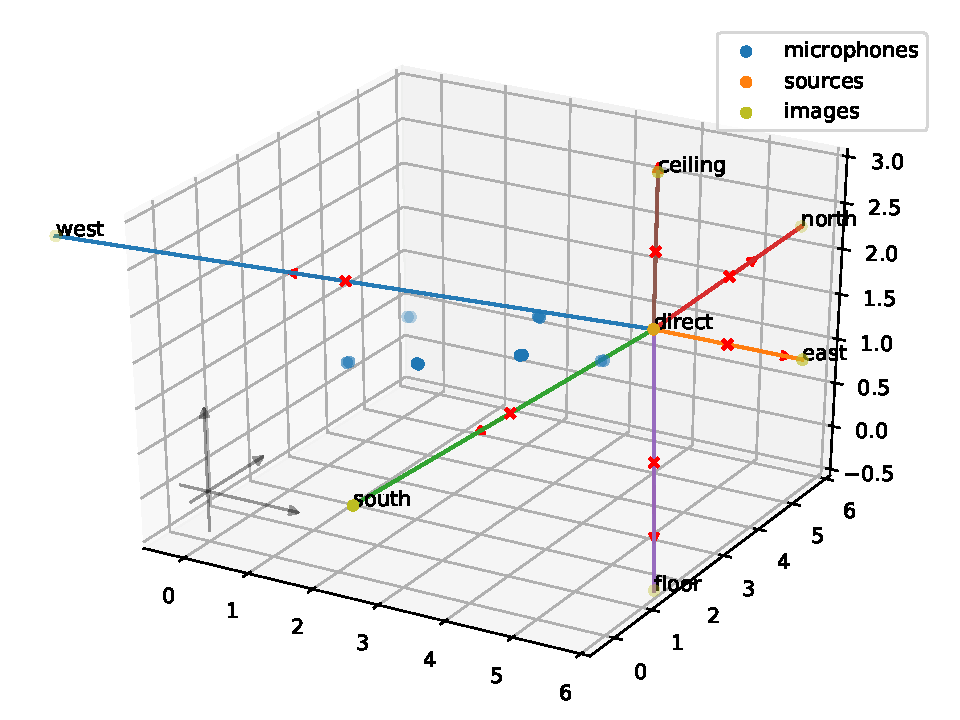
\includegraphics[width=0.49\textwidth]{figures/estimated_image}}
%     \hfill
%     \subfigure{
%         \includegraphics[width=0.49\textwidth]{figures/estimated_reflector}}

%     \caption{Images source estimation (right) and corresponding reflector estimation (left) for one of the sound sources in the dataset.}
%     \label{fig:wall_rec}
% \end{figure}

\begin{figure}

        \includegraphics[width=\linewidth]{figures/dechorate/estimated_reflector}

    \caption{Images source estimation and reflector estimation for one of the sound sources in the dataset.}
    \label{fig:wall_rec}
\end{figure}

\section{Conclusions and Perspectives}

This paper introduced a new database of room impulse responses featuring accurate annotation of early echoes and microphone positions. These data can be used to test methods in the room geometry estimation pipeline and in echo-aware audio signal processing. In particular, robustness of these methods can be validated against different levels of $\RT$, SNR or even early echo density.